\chapter{Theory}
\begin{comment}
This chapter will contain the essential theory for the thesis. 

As the authors did a literature review as a pre-study for this project, some subchapters will be re-used as the theory is still highly relevant for this thesis. 
\end{comment}
Chapter 2 of the thesis introduces the challenges of using machine learning with graphs and how GCNs have emerged as a solution to these challenges. The chapter describes the core of GCNs, the graph convolution operation, and how it aggregates local information from neighbouring nodes to generate a new representation for each node. The chapter also introduces \Gls{AutoML}, an emerging area of machine learning that seeks to automate designing optimal machine learning architectures. Finally, the chapter provides an overview of NAS, a sub-field of AutoML that aims to automate creating of high-performing neural networks and HAR. 

\section{Deep Learning} 
Deep learning, a subfield of machine learning, has gained significant attention in recent years due to its ability to learn hierarchical representations from raw data, especially in domains such as computer vision, natural language processing, and speech recognition. This contrasts conventional machine-learning techniques, which are limited in processing the same \autocite{lecun2015deep}. 

The core building blocks of deep learning are \Gls{ANN} inspired by the biological neural networks found in the human brain. \glspl{ANN} consist of interconnected layers of artificial neurons called nodes, each receiving input from previous layers, processing the information, and propagating the output to the subsequent layers. Deep learning architectures typically involve multiple layers of these interconnected nodes, hence the term "deep" \autocite{goodfellow2016deep}.

One key advantage of deep learning over traditional machine learning techniques is its ability to automatically learn and extract features from raw data without relying on manual feature engineering. This process, called representation learning, enables deep learning models to understand hierarchical representations of the input data, with each layer capturing increasingly abstract and complex features \autocite{bengio2013representation}. This capability has led to breakthrough performance improvements in various applications, including image classification, natural language understanding, and speech recognition \autocite{krizhevsky2017imagenet}.
\subsection{Neural Networks}\label{neuralnet}
Neural Networks are a part of neurocomputing, a field of study that aims to develop computational systems inspired by the human brain's structure and function. For example, pattern recognition, motor control, vision, flexible inference, intuition, and accurate guessing are all skills the brain is particularly adept at, which is what neural networks aim to emulate \autocite{anderson1995introduction}. 

At a high level, a neural network is a collection of interconnected nodes (called "neurons") arranged in layers. The input layer receives input data, which is passed through one or more hidden layers before the output from the final layer.

The basic unit of a neural network is a neuron, which receives input from other neurons or the input layer. The neuron then applies a mathematical function to this input, producing an output sent to other neurons in the next layer. The most commonly used function is the sigmoid function, given in \cref{eq:sigmoid}. 

\begin{equation}
    \sigma(z) = \frac{1}{1+e^{-z}}
    \label{eq:sigmoid}
\end{equation}

where $z$ is the input to the neuron, the sigmoid function has the valuable property that its output is always between 0 and 1, which can be interpreted as a probability.

The output of a neuron is determined by the weights and biases associated with its inputs. Each input is multiplied by a weight, and these weighted inputs are summed together with a bias term to produce the neuron's input, as shown in \cref{eq:z}. 

\begin{equation}
    z = \sum_{i=1}^n w_i x_i + b
    \label{eq:z}
\end{equation}

where $w_i$ is the weight associated with the $i$th input, $x_i$ is the value of the $i$th input, $n$ is the number of inputs, and $b$ is the bias term.

\Cref{eq:y} exhibits the neuron output when applying the sigmoid function to the input.

\begin{equation}
    y = \sigma(z)
    \label{eq:y}
\end{equation}

During the training process, which comprises feeding training data through the network (illustrated in \cref{fig:nn}) and modifying the weights and biases based on the difference between the predicted output and the actual output, the weights and biases of a neural network are changed. Usually, a gradient descent optimisation technique is used to carry out this operation.

\begin{figure}[h]
\resizebox{\textwidth}{!}{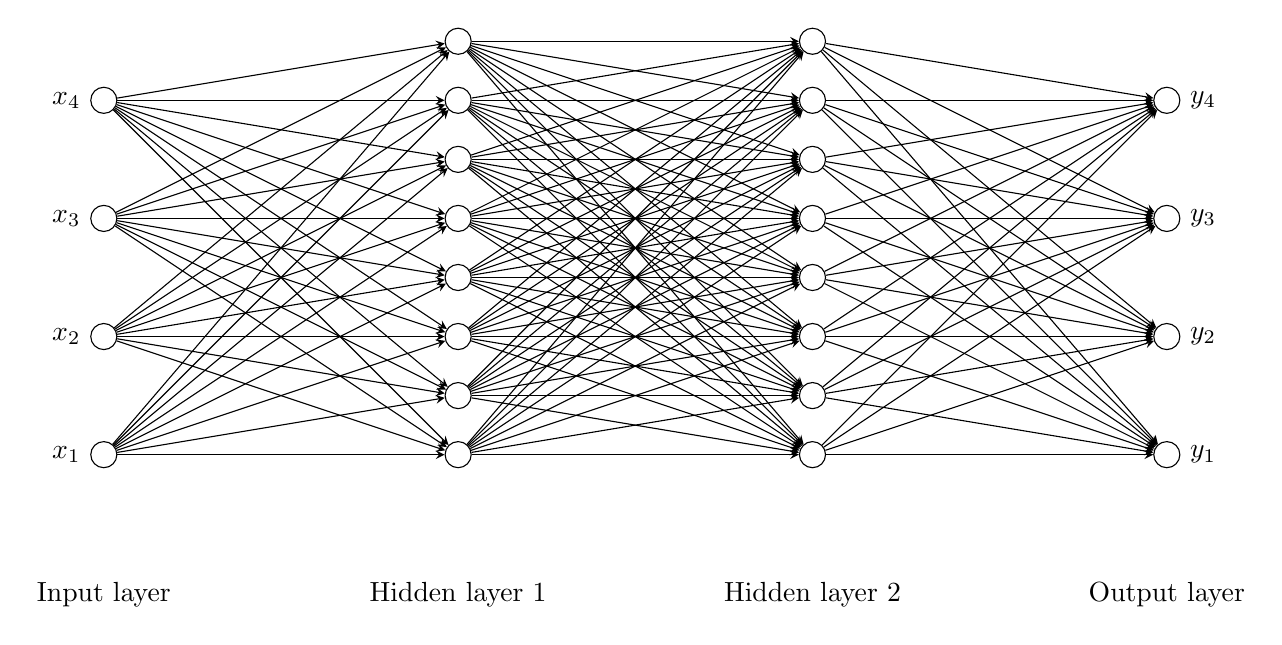
\begin{tikzpicture}[x=3cm, y=1.5cm, >=stealth]
    
    % Input layer nodes
    \foreach \i in {1,...,4} {
        \node[draw, circle] (input-\i) at (0, \i) {};
    }
    
    % First hidden layer nodes
    \foreach \i in {1,...,8} {
        \node[draw, circle] (hidden1-\i) at (1.5, 0.5 + 0.5*\i) {};
    }
    
    % Second hidden layer nodes
    \foreach \i in {1,...,8} {
        \node[draw, circle] (hidden2-\i) at (3, 0.5 + 0.5*\i) {};
    }
    
    % Output nodes
    \foreach \i in {1,...,4} {
        \node[draw, circle] (output-\i) at (4.5, \i) {};
    }

    % Input layer labels
    \foreach \i in {1,...,4} {
        \node[left] at (input-\i.west) {$x_{\i}$};
    }
    
    % Output layer labels
    \foreach \i in {1,...,4} {
        \node[right] at (output-\i.east) {$y_{\i}$};
    }
    
    % Connect input to first hidden layer
    \foreach \i in {1,...,4} {
        \foreach \j in {1,...,8} {
            \draw[->] (input-\i) -- (hidden1-\j);
        }
    }
    
    % Connect first hidden layer to second hidden layer
    \foreach \i in {1,...,8} {
        \foreach \j in {1,...,8} {
            \draw[->] (hidden1-\i) -- (hidden2-\j);
        }
    }
    
    % Connect second hidden layer to output
    \foreach \i in {1,...,8} {
        \foreach \j in {1,...,4} {
            \draw[->] (hidden2-\i) -- (output-\j);
        }
    }
    
    % Layer labels
    \node[below] at (0, 0) {Input layer};
    \node[below] at (1.5, 0) {Hidden layer 1};
    \node[below] at (3, 0) {Hidden layer 2};
    \node[below] at (4.5, 0) {Output layer};

\end{tikzpicture}}
\caption{Illustration of Neural Network}
\label{fig:nn}
\end{figure}

\section{Graph Convolutional Networks}

Graphs are ubiquitous structures representing complex systems, including social networks, biological networks, and transportation systems \autocite{scarselli2008graph}. They consist of nodes and edges, representing the many entities and relationships between them. Despite their widespread use, graphs pose unique challenges in machine learning due to their irregular structure, which makes it difficult to apply conventional learning techniques that rely on fixed-size inputs and Euclidean data representations \autocite{battaglia2018relational}.

\Gls{GNN} has emerged as a solution to these challenges, generalising deep learning techniques to graph-structured data \autocite{gori2005new}. Among GNNs, GCNs have become particularly popular owing to their ability to perform localised and efficient convolutions on graph data \autocite{DBLP:journals/corr/KipfW16}. GCNs extend the concept of convolution from grid-like structures, such as images, to irregular graph structures, enabling the extraction of meaningful features from graph data while preserving their spatial relationships \autocite{bronstein2017geometric}. 

\subsection{Graph Convolutions}
The core of GCNs lies in the graph convolution operation, which aims to aggregate local information from neighbouring nodes to generate a new representation for each node. The main idea is to perform a weighted sum of the feature vectors of a node and its neighbours, where the weights are determined by the edge weights or some measure of node similarity. This aggregation scheme allows GCNs to learn node representations that effectively capture the local graph structure. The \cref{eq:kiph}, found in \autocite{DBLP:journals/corr/KipfW16}, shows how the graph convolution operation are mathematically described.

\begin{equation*} 
    \bm{H}^{l+1} = \sigma(\bm{\hat{D}}^{-\frac{1}{2}} \bm{A} \bm{\hat{D}}^{-\frac{1}{2}} \bm{H}^{l} \bm{W}^{l} )
    \label{eq:kiph}
\end{equation*}


The components in \cref{eq:kiph} are defined as follows:

$H^{(l+1)}$ stands for the updated node representations (features) at layer $(l+1)$, while $H^{(l)}$ indicates the node features at layer $l$. $H^{(0)}$ is the input feature matrix for the first layer. The graph's adjacency matrix, represented by $A$, is modified to incorporate self-connections. This is achieved by adding a diagonal matrix with ones to the original adjacency matrix $A$, ensuring that the node's features are considered during the aggregation process.

The degree matrix, denoted by $\hat{D}$, corresponds to the modified adjacency matrix $\hat{A}$. It is a diagonal matrix wherein each diagonal entry signifies the degree (number of connections) of the corresponding node. The learnable weight matrix at layer $l$ is represented by $W^{(l)}$ and is employed to linearly transform the node features at each layer.

Lastly, the activation function $\sigma$ introduces non-linearity to the model. Typical choices for activation functions are ReLU, sigmoid, and tanh.





\section{Automated Machine Learning (AutoML)}\label{section:automl}
\glsreset{AutoML}

Fields such as computer vision, speech recognition, and natural language processing have seen significant progress, primarily due to the development and application of deep learning techniques in recent years. However, despite these advancements, designing optimal machine learning architectures remains complex and time-consuming for data scientists. \Gls{AutoML} is an area that seeks to automate this process.  

\subsection{Hyperparameter Optimisation}\label{subsection:hyperparameter-optimization}
Hyperparameter optimisation is a critical component of the \gls{AutoML} pipeline. Machine learning algorithms often contain hyperparameters that control their behaviour, and their optimal values are not learned directly from the training data. Instead, these parameters need to be set manually or searched for systematically. Traditional techniques for hyperparameter tuning include grid search, random search, and manual tuning. However, these approaches can be computationally expensive and inefficient.
\gls{AutoML} aims to streamline this process by employing advanced techniques such as Bayesian optimisation, evolutionary algorithms, and gradient-based methods. These methods can efficiently explore the hyperparameter space and identify suitable configurations, ultimately leading to improved model performance and reduced computational cost \autocite{bergstra2011algorithms, snoek2012practical}.

\subsection{Meta-learning}\label{subsection:meta-learning}
Meta-learning, also called "learning to learn", is another crucial component of \gls{AutoML}. The central idea is to utilise prior knowledge gained from solving multiple related tasks to improve the learning efficiency and generalisation ability on new tasks. This is achieved by learning a model or an algorithm that can adapt quickly to novel tasks with limited data.
In the context of \gls{AutoML}, meta-learning can be employed in various ways. One popular approach is to use meta-learning for transfer learning, wherein a pre-trained model is fine-tuned on a new task with limited available data \autocite{pan2010survey}. Another application of meta-learning is hyperparameter optimisation, where a meta-model can be trained to predict the performance of different configurations across various tasks. This knowledge can guide the search for optimal hyperparameters more efficiently \autocite{swersky2014freeze}.
\section{Neural Architecture Search (NAS)} \label{section:nas}
\glsreset{NAS}
Most neural architectures are created by specialists, which is labour-intensive and susceptible to other weaknesses. Subsequently, a way of automatically designing and developing such algorithms has been a research field for a couple of years. Thus, \gls{NAS} aims to automate the previously manual process of designing architectures \autocite{elsken2019neural}. Consequently, \gls{NAS} is a sub-field of \gls{AutoML} (\cref{section:automl}). 

Given the search space $F$, a training set $D_{\text{train}}$, validation set $D_{\text{valid}}$ and an evaluation metric $M$, the \gls{NAS} problems aims at finding an optimal architecture $f^* \in F$ with the best metric $M^*$ on the validation set $D_{\text{valid}}$. This can be written mathematically as 

\begin{equation*}
    f^* = \text{argmax}_{f \in F} M(f(\theta^*), D_{\text{valid}}) 
\end{equation*}

\begin{equation*}
    \theta^* = \text{argmin}_{\theta} L(f(\theta), D_{\text{train}}), 
\end{equation*}

where $\theta^*$ is the learned parameters for the architecture $f$ and $L$ is the loss function \autocite{zhou2019auto}. 

\Cref{fig:nas_overview} shows how \gls{NAS} works. The search space gives the algorithm a constraint regarding how it can be developed by defining a set of architectural choices the model might use. For example, the constraint might be different operations such as convolution, fully connected and pooling. One might argue that this is vital as selecting the search space can reduce the search's complexity, which is crucial to produce an acceptable model \autocite{kyriakides2020introduction}.

\begin{figure}[h]
    \centering
    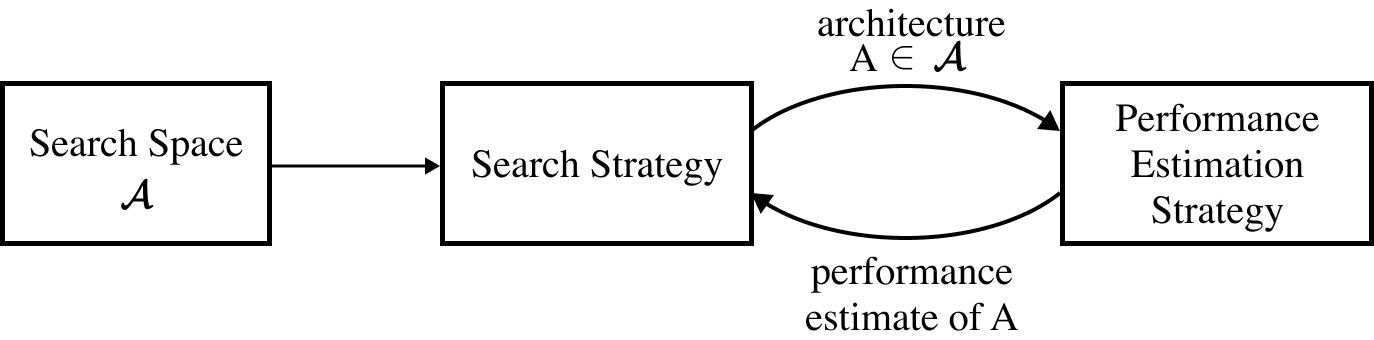
\includegraphics[width=12cm]{figures/NAS_overview.png}
    \caption{An overview of the different methods in NAS \autocite{elsken2019neural} }
    \label{fig:nas_overview}
\end{figure}

After defining a search space for the given problem, a \gls{NAS} search algorithm will specify how to analyse the search space and propose a set of candidate architectures. This introduces the exploration-exploitation trade-off, which indicates that selecting an appropriate optimisation technique is vital because we want to find a global optimum and ensure that the search space is sufficiently investigated \autocite{kyriakides2020introduction}. 

The framework must perform performance estimation for each candidate architecture to adjust the search strategy. The simplest solution is to train and validate the model, which is too computationally expensive because it usually involves training days for \gls{GPU}. Furthermore, many hours of training require a lot of energy, which has a high environmental cost. Another downside of training the architectures is that it will limit the number of architectures the search algorithm might discover. As a result, methods simplifying this phase have been undergoing heavy research \autocite{elsken2019neural}. 

Another goal of NAS is to discover optimal architectures concerning ...

\subsection{Challenges}
\subsubsection{Computational power}
The most straightforward approach to determine the performance of a neural network is to train it until the validation accuracy has converged against a value or has been run for a fixed amount of epochs. However, training thousands of architectures may require hundreds or more GPU days \autocite{ren2021comprehensive}. The computational power required may be available for larger companies with plentiful resources. However, for most users, this is computationally infeasible. As a result, the necessary computational power is considered a significant challenge for NAS. 

\subsubsection{Black-box optimisation and lack of interpretability}
NAS algorithms often treat the architecture search space as a black box, meaning they cannot access the internal workings of the searched model architectures. This can make it difficult to incorporate domain knowledge or bias the search towards certain types of architectures. This results in difficult-to-interpret architectures, making it challenging to understand how they make predictions or identify potential problems with the architecture. \autocite{https://doi.org/10.48550/arxiv.1806.09055}

\subsection{Search Space}
When searching for a high-performing architecture, there are infinite variations that one might investigate. As a result, one defines a search space that gives the search algorithm constraints regarding what kind of combinations it might examine. Prior knowledge of what kind of search space is effective on specific tasks may reduce the size, but it has the disadvantage of introducing human bias in the search space \autocite{elsken2019neural}.  

Global search space is a way in which it tries to combine all possible operations to create chain-structured (sequential) networks. Then, the search space has the following parameters:
\begin{itemize}
    \item the number of layers
    \item the type of each operation
    \item the hyperparameters of each operation, namely kernel size, number of filters etc. 
\end{itemize}

Such a network can be described as a sequence of $n$ layers, where layer $L_i$ takes $L_{i-1}$ as input. However, this sort of search space is enormous and very expensive. 

Cell-based representations were inspired by successful architectures using repeated modules (Inception, ResNet). NASNet paper \autocite{DBLP:journals/corr/ZophVSL17}, is one of the most popular cell- or block-based approaches. Cell-based representations differ from global search space because they search for cells or blocks instead of whole architectures \autocite{elsken2019neural}. \cite{DBLP:journals/corr/ZophVSL17} learns two sorts of cells; a normal cell which performs feature extraction (preserving dimensionality), and a reduction cell which reduces the dimensionality. By stacking such cells, we get the final architecture, as shown in \cref{fig:cells}. 

\clearpage

\begin{figure}
    \centering
    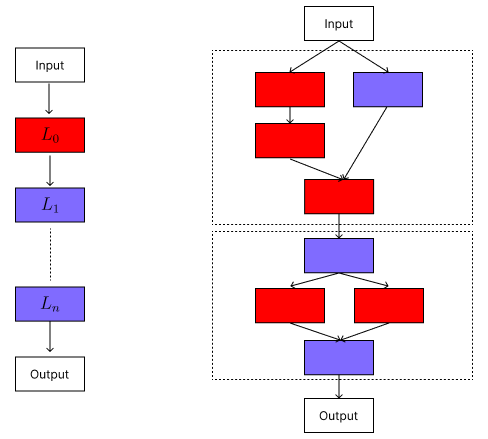
\includegraphics[width=8cm]{figures/cells.png}
    \caption{Left: chain-structured network, right: cells combined into an architecture}
    \label{fig:cells}
\end{figure}

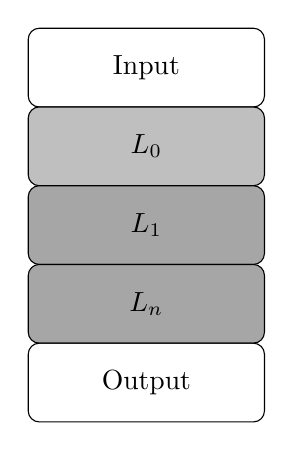
\begin{tikzpicture}
    \node (input) [rectangle, rounded corners, text centered, draw=black, minimum width=3cm, minimum height=1cm] {Input};
    \node (l0) [rectangle, rounded corners, text centered, draw=black, fill=gray!50, minimum width=3cm, minimum height=1cm, below of=input] {$L_0$};
    \node (l1) [rectangle, rounded corners, text centered, draw=black, fill=gray!70, minimum width=3cm, minimum height=1cm, below of=l0] {$L_1$};
    \node (ln) [rectangle, rounded corners, text centered, draw=black, fill=gray!70, minimum width=3cm, minimum height=1cm, below of=l1] {$L_n$};
    \node (output) [rectangle, rounded corners, text centered, draw=black, minimum width=3cm, minimum height=1cm, below of=ln] {Output};
\end{tikzpicture}

\clearpage

\subsubsection{Directed Acyclic Graphs}
\glsreset{DAG}
\Gls{DAG} is often used in \gls{NAS} to represent the structure of a neural network. In this context, the graph's vertices represent different operations or layers in the network, and the graph's edges represent the data flow between these operations. This allows researchers to efficiently represent and manipulate the structure of a neural network during the search process.

One of the main advantages of using \glspl{DAG} in \gls{NAS} is that they provide a convenient way to encode the constraints on the network architecture. For example, a \gls{DAG} can enforce the requirement that a neural network must have a certain number of layers or that individual layers must be connected in a specific way. This can help ensure that the search process only considers valid network architectures, which can speed up the search and improve its accuracy \autocite{https://doi.org/10.48550/arxiv.1806.09055}. 

In addition to representing the structure of a neural network, \glspl{DAG} can also represent the search space over which the architecture search algorithm operates. This allows the algorithm to explore different network architectures efficiently and evaluate their performance, ultimately discovering novel and effective network architectures \autocite{inproceedings}. 

\subsection{Search Strategies}

\subsubsection{Random Search}
Random search is the most naive search strategy, and it will simply randomly pick a good architecture based on the search space. Therefore, the method is relatively fast and does not require any learning model. A random search may be effective if a search space is well constructed.  

\subsubsection{Reinforcement Learning}
On the very basic, reinforcement learning is an area within machine learning in which an agent learns behaviour by some trial-and-error interaction with a dynamic environment \autocite{kaelbling1996reinforcement}. One can consider \gls{NAS} a reinforcement problem by looking at the creation of the architecture as the agent's action, in which the action space is the problem's search space. The agent gets rewarded depending on the performance of the trained architecture. There are numerous approaches to representing an agent's policy, such as a recurrent neural network, proximal policy optimisation and q-learning \autocite{elsken2019neural}. 

\subsubsection{Evolutionary algorithms}
Evolutionary algorithms are techniques used in optimisation and search methods. It is a subset of \gls{EC} and is an effective way of problem-solving for often encountered global optimisation problems because of its adaptable character \autocite{7955308}. Evolutionary algorithms in \gls{NAS} randomly select $N$ initialised models and then assess performance by the given evaluation strategy. The best models are chosen as parents, and new models have mutated clones of the parents, which are re-evaluated. Finally, the worst $N$ models are removed from the population to make room for new offspring \autocite{https://doi.org/10.48550/arxiv.1703.01041}. 

\subsubsection{Bayesian optimisation}
\Gls{BO} has been a popular approach for hyperparameter optimisation \autocite{elsken2019neural}. In general, \gls{BO} optimises expensive functions to evaluate, such as the performance of architectures. This is a global optimisation problem that \gls{BO} tries to solve. Given a costly to evaluate function $f$, \gls{BO} aims at finding its optimal score within some domain $x$ \autocite{kandasamy2018neural}. In other words, \gls{BO} pursues to calculate $a^* = arg min_{a \in A} f(a)$, where A is the given search space, and $f(a)$ is the performance function of the neural network after training the architecture $a$ for a fixed number of iterations \autocite{white2021bananas}.  

\subsection{Performance Estimation}
\subsubsection{Performance Predictors}\label{sec:performancepredictors}
As mentioned in \cref{section:nas}, \gls{NAS} aims to automate the process of designing high-performing neural networks. However, this often requires training all the candidate networks, either partly or wholly, to get the accuracy of the neural networks. In most cases, this is an infeasible approach when the search space is big, which is why performance predictors are introduced \autocite{akhauri2022evolving}. 

Any function that forecasts the eventual accuracy or ranking of architectures without fully training the architecture is referred to as a performance predictor $f$. Therefore, the performance predictor's function should take significantly less time than training and validating the neural network fully and have a high correlation or rank correlation with the validation error \autocite{white2021powerful}. 

A performance predictor is defined by two main routines - initialisation and query. The initialisation routine does some general pre-computation, often before the \gls{NAS} algorithm. For model-based methods, the initialisation routine consists of fully training a set of architectures to get data points. Then, the query routine will output the predicted accuracy with the architecture details as input \autocite{white2021powerful}. 

There exist multiple categories of performance predictors:

\begin{table}[h]
\caption{List of performance predictors}
\centering
\begin{tabular}{|l}
Model-based (trainable) methods \\
\cellcolor{verylightgray}Learning curve-based methods    \\
Hybrid methods                  \\
\cellcolor{verylightgray}Zero-cost proxies               \\
Weight sharing methods         
\end{tabular}
\end{table}

\subsubsection{Zero-Cost Proxies}\label{subsec:zerocost}
Zero-cost proxies are a class of performance predictors. The name zero-cost comes from analysing a neural network at initialisation, indicating that it costs 'zero' to generate the score. At the same time, the predicted accuracy is closely correlated with the actual accuracy. 

By performing a single forward/backward propagation pass using a single minibatch of data, zero-cost proxies methods can score a neural network \autocite{akhauri2022evolving}. The intuition is that one can measure the 'trainability' of a neural network by looking at the initial gradient flow. 

The paper \textit{Zero-Cost Proxies for Lightweight NAS}, \autocite{abdelfattah2021zero} showed the usefulness of a range of zero-cost proxies inspired by the pruning-at-initialisation literature. Each method can be divided into two categories - data-independent or data-dependent. 

Data-dependent zero-cost proxies use data to generate the score, whereas data-independent will not use the dataset in principle. Sometimes, it is used to set dimensions \autocite{colin2022adeeperlook}. \Cref{tab:zcproxies} lists data-independent and data-dependent zero-cost proxies. However, this collection is not exhaustive, and additional zero-cost proxies are not included. 


\begin{table}[ht]
    \caption{Different zero-cost proxies within the two categories data-independent and data-dependent}
    \centering
    \begin{tabular}{l|l}
    \textbf{Data-independent}         & \textbf{Data-dependent} \\ \hline
    Synflow & EPE-NAS                   \\
    \cellcolor{verylightgray}Zen-score                       & \cellcolor{verylightgray}Fisher                    \\
    GenNAS                          & Grad-norm                 \\
    \cellcolor{verylightgray}number of parameters in network & \cellcolor{verylightgray}Grasp                                 
    \end{tabular}
    \label{tab:zcproxies}
\end{table}


 
\section{Human Activity Recognition}

HAR is a method that interprets the human body's gestures or motions via sensors, accelerometers or videos and uses these to predict human action \autocite{jobanputra2019human}. Like many other computer vision tasks, HAR can be supervised and unsupervised, where supervised training requires a large amount of data \autocite{ann2014human}. Therefore, we can classify HAR into two problems; the localisation problem and the recognition problem. The localisation problem concerns where something is in the video, whereas the recognition problem concerns the type of action we see \autocite{vrigkas2015review}. 

HAR may be concerned about videos which bring several challenges along. Due to problems like background clutter, partial occlusion, and changes in scale and frame resolution, capturing the specific action of a human within a video is a challenging task \autocite{vrigkas2015review}. However, modelling the human body as three-dimensional data is another approach that has emerged in recent years. The human body can be divided into connecting joints forming a three-dimensional structure.  
